\section{Auswertung}
\label{sec:Auswertung}

\subsection{a)}
Nachfolgend finden sich die aufgenommenen Messdaten ausgedrückt in SI-Einheiten. Zu den beiden Drücken $p_a$ und $p_b$ wurde jeweils $1 bar$ ($1\cdot10^5 Pa$) addiert. (vgl. \cite{Anleitung})
\begin{table}
  \centering
  \caption{Messdaten}

  \label{tab:Messdaten}
\begin{tabular}{cccccc}
\toprule
$\frac{t}{s}$ & $\frac{T_1}{K}$ & $\frac{T_2}{K}$& $\frac{p_b\cdot10^5}{Pa}$ & $\frac{p_a\cdot10^5}{Pa}$ & $\frac{P}{W}$ \\
\midrule
0.0 & 293.85 & 293.65 & 4.7 & 5.02 & 0.0 \\
60.0 & 293.95 & 293.65 & 6.7 & 4.22 & 119.0 \\
120.0 & 294.45 & 293.65 & 7.0 & 4.38 & 120.0 \\
180.0 & 295.75 & 293.65 & 7.1 & 4.43 & 123.0 \\
240.0 & 297.35 & 292.95 & 7.3 & 4.43 & 124.0 \\
300.0 & 298.65 & 292.05 & 7.5 & 4.39 & 123.0 \\
360.0 & 299.85 & 291.25 & 7.8 & 4.3 & 122.0 \\
420.0 & 300.55 & 290.35 & 8.0 & 4.21 & 121.0 \\
480.0 & 302.15 & 289.55 & 8.1 & 4.17 & 121.0 \\
540.0 & 303.25 & 288.85 & 8.3 & 4.02 & 120.0 \\
600.0 & 304.35 & 288.05 & 8.4 & 3.97 & 119.0 \\
660.0 & 305.25 & 287.35 & 8.7 & 3.88 & 119.0 \\
720.0 & 306.25 & 286.65 & 8.9 & 3.8 & 119.0 \\
780.0 & 307.15 & 286.05 & 9.0 & 3.77 & 119.0 \\
840.0 & 308.05 & 285.45 & 9.1 & 3.7 & 120.0 \\
900.0 & 308.95 & 284.95 & 9.3 & 3.63 & 120.0 \\
960.0 & 309.75 & 284.35 & 9.6 & 3.6 & 120.0 \\
1020.0 & 310.55 & 283.85 & 9.8 & 3.58 & 121.0 \\
1080.0 & 311.45 & 283.35 & 10.0 & 3.53 & 121.0 \\
1140.0 & 312.25 & 282.85 & 10.1 & 3.49 & 121.0 \\
1200.0 & 313.15 & 282.35 & 10.3 & 3.43 & 122.0 \\
1260.0 & 313.95 & 281.95 & 10.4 & 3.42 & 122.0 \\
1320.0 & 314.65 & 281.55 & 10.6 & 3.4 & 122.0 \\
1380.0 & 315.35 & 281.15 & 10.8 & 3.39 & 122.0 \\
1440.0 & 316.05 & 280.75 & 10.9 & 3.37 & 122.0 \\
1500.0 & 316.75 & 280.45 & 11.1 & 3.35 & 122.0 \\
1560.0 & 317.45 & 280.15 & 11.2 & 3.33 & 122.0 \\
1620.0 & 318.05 & 279.85 & 11.3 & 3.3 & 122.0 \\
1680.0 & 318.65 & 279.55 & 11.5 & 3.28 & 122.0 \\
1740.0 & 319.25 & 279.35 & 11.7 & 3.25 & 122.0 \\
1800.0 & 319.85 & 278.35 & 11.8 & 3.23 & 122.0 \\
1860.0 & 320.55 & 277.25 & 11.9 & 3.22 & 122.0 \\
1920.0 & 321.05 & 276.85 & 12.1 & 3.21 & 122.0 \\
1980.0 & 321.55 & 276.55 & 12.2 & 3.21 & 122.0 \\
2040.0 & 322.05 & 276.25 & 12.4 & 3.2 & 122.0 \\
2100.0 & 322.65 & 276.05 & 12.5 & 3.2 & 122.0 \\
2160.0 & 323.15 & 276.05 & 12.7 & 3.2 & 122.0 \\
\end{tabular}

\end{table}

\newpage
\subsection{b)}
Eine nicht-lineare Ausgleichsrechnung mittels curvefit mithilfe der Näherungsfunktion $T(t) = 
\frac{At^{\alpha}}{1 + Bt^{\alpha}} + C$ ergibt die folgenden Parameter

für T1
\begin{table}
\begin{tabular}{cc}
col0 & col1 \\
A& 0.00628783578154 \pm 0.00149293305498 \\
$\alpha$& 1.19703458148 \pm 0.0360058939096 \\
B& 0.0001090619383 \pm 2.08039537226e-05 \\
C& 293.237543897 \pm 0.166671854986 \\
\end{tabular}
\end{table}

für T2
\begin{table}
\begin{tabular}{cc}
col0 & col1 \\
A&-0.00133382194218 \pm 0.00104923580266 \\
$\alpha$ &1.34714994906 \pm 0.118067658101 \\
B&4.09937384238e-05 \pm 2.72288576068e-05 \\
C& 294.320491079 \pm 0.29104291577 \\
\end{tabular}
\end{table}

\begin{figure}
  \centering
  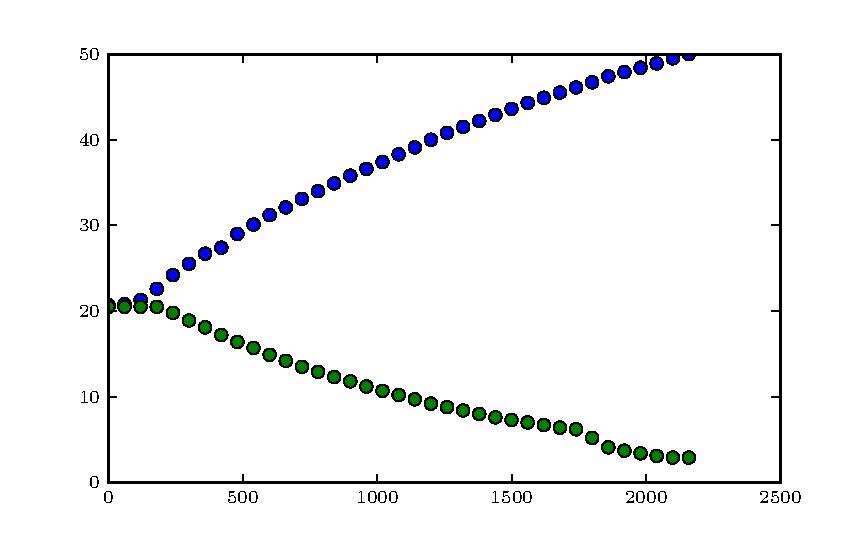
\includegraphics{plot.pdf}
  \caption{Plot}
  \label{fig:plot}
\end{figure}

\subsection{c)}
Im Auswertungsteil c) sollen die Differentialquotienten $\frac{\symup{d}T_{1,2}}{\symup{d}t}$
für vier verschieden Temperaturen $T_i$ berechnet werden.

Nun gilt ja für die beiden Temperaturen $T_1$ und $T_2$ die Näherungsfunktion
\begin{equation}
	T_i(t) = \frac{A_i t^{\alpha_i}}{1 + B_i t^{\alpha_i}} + C_i
\end{equation}
Damit erhält man für den Differentialquotienten
\begin{equation}
	\frac{\symup{d}T_i}{\symup{d}t} = \frac{\alpha_i A_i t^{\alpha_i - 1}}{(1 + B_i t^{\alpha_i})^2}
\end{equation}
Es werden die vier Temperaturen zugehörig zu den Zeiten 300s, 600s, 900s und 1200s betrachtet.
Für $T_1$ ergeben sich die Werte 
\begin{table}
\begin{tabular}{cc}
Zeit $t$ in s & Temperatur $T_1$ in Grad Celsius \\
	300 & 25,5 \\
	600 & 31,2 \\
	900 & 35,9 \\
	1200 & 40,0 \\
\end{tabular}
\end{table}





